\documentclass[UTF8,a4paper,12pt]{ctexart}

\usepackage[a4paper,margin=2.2cm]{geometry}
\usepackage{amsmath,amssymb}
\usepackage{graphicx}
\usepackage{booktabs}
\usepackage{float}
\usepackage{array}
\usepackage{xurl}
\usepackage[colorlinks=true,linkcolor=black,citecolor=black,urlcolor=blue]{hyperref}
\usepackage{setspace}
\usepackage{titlesec}
\usepackage{fancyhdr}
\usepackage{subcaption}
\usepackage{tikz}
\usetikzlibrary{positioning,arrows.meta,fit,backgrounds}

\pagestyle{fancy}
\fancyhf{}
\cfoot{\thepage}
\renewcommand{\headrulewidth}{0pt}

\setlength{\parskip}{0.35em}
\setlength{\parindent}{2em}
\linespread{1.18}

\titleformat{\section}{\Large\bfseries}{\thesection}{0.8em}{}
\titleformat{\subsection}{\large\bfseries}{\thesubsection}{0.8em}{}

\newcommand{\maybeincludegraphics}[2][]{%
\IfFileExists{#2}{\includegraphics[#1]{#2}}{%
\fbox{\parbox{0.82\linewidth}{\centering Missing figure: \texttt{\detokenize{#2}}}}%
}%
}

\title{基于 2D U-Net 的 MRI T1 加权脑部图像去噪}
\author{洪家权 \quad 23307110248@m.fudan.edu.cn}
\date{}

\begin{document}

\maketitle

% \begin{abstract}
% 本实验面向 MRI T1 加权脑部图像去噪任务，采用监督学习方式训练 2D U-Net 模型，将带噪声的轴向 T1 切片映射为对应的干净 T1 切片。数据集共包含 600 个 case，每个 case 由一对 noisy 与 clean 3D NIfTI 体积组成。实验首先在 case 级别完成训练集、验证集和测试集划分，再对体数据进行轴向切片提取、脑组织过滤、分位数归一化和统一尺寸 padding。模型结构采用典型的编码器—解码器 U-Net，利用跳跃连接融合浅层空间细节与深层语义特征。训练阶段使用 L1 损失与 SSIM 损失的联合目标，在保持像素级重建精度的同时约束图像结构一致性。最终模型在 60 个测试 case 上取得约 45.3 dB 的 case 级平均 PSNR 和约 0.989 的 case 级平均 SSIM，说明模型能够有效去除 T1 图像噪声，并保持较好的结构重建质量。
% \end{abstract}

\section{简介}

医学图像去噪的核心目标是在抑制噪声的同时尽可能保留解剖结构、组织边界和局部纹理信息。对于 MRI T1 加权脑部图像而言，噪声会影响灰白质边界、脑室结构和皮层形态的观察，也会干扰后续分割、配准或定量分析任务。因此，本实验将 MRI T1 去噪建模为一个监督式图像到图像重建问题，即输入带噪声的 T1 轴向切片，输出同一受试者对应位置的干净 T1 切片。

本实验使用的数据集包含 600 个 case，每个 case 对应一对三维 NIfTI 体积文件，分别为 noisy T1 图像与 clean T1 图像。由于原始数据是三维体数据，而实验采用 2D U-Net 模型，因此预处理阶段沿轴向方向将体数据切割为二维切片，并过滤掉主要由背景组成的无效切片。为了避免同一受试者的相邻切片同时出现在训练集与测试集中造成数据泄漏，数据划分在 case 级别完成，而不是在 slice 级别随机划分。

方法上，本实验选择 2D U-Net 作为主体网络。U-Net 通过编码器逐步扩大感受野，通过解码器逐步恢复空间分辨率，并借助跳跃连接将高分辨率浅层特征传递到对应的解码阶段。这一结构适合医学图像重建任务，因为去噪既需要全局上下文判断噪声模式，也需要保留局部结构边界。训练目标采用 L1 损失与 SSIM 损失的加权组合，其中 L1 损失约束像素级误差，SSIM 损失约束局部亮度、对比度和结构相似性。最终测试结果显示，两次训练运行的测试性能高度一致，说明模型收敛稳定，且在未见过 case 上具有较好泛化能力。

\section{实验设计}

\subsection{数据集划分与预处理}

原始数据集共包含 600 个 case，每个 case 包含一个 noisy T1 体积和一个 clean T1 体积，两者构成一一对应的监督学习样本。实验沿轴向方向对三维体数据进行切片提取，将每个体积转换为若干二维图像。不同 case 的切片数量并不完全一致，全部数据切片总量约为 90,247 张。为了减少空背景切片对训练的干扰，实验基于 clean 切片进行脑组织过滤。具体而言，对每张 clean 切片统计像素值大于 50.0 的区域占比；若该占比不低于 5\%，则认为该切片包含有效脑组织并予以保留，否则将其视为主要由空气或无效背景构成的切片并丢弃。

归一化阶段采用分位数截断和线性映射。对于每个 case，首先根据 noisy 体积的 0.5\% 与 99.5\% 分位数确定截断上下界，然后将 noisy 体积裁剪到该范围并线性映射至 $[0,1]$。对应的 clean 体积使用同一组上下界进行归一化，从而保证 noisy 与 clean 之间的 paired 关系不被破坏。相较于直接使用全局最小值和最大值，分位数归一化可以减弱极端像素值对强度尺度的影响，同时保留同一 case 内的相对灰度结构。

尺寸处理方面，实验遍历全体切片后确定统一输入大小，并将切片高宽向上补齐至 16 的倍数，最终所有切片均被 zero-padding 至 $256\times256$。padding 只在边缘区域补零，不改变原始图像区域的像素值。训练、验证和测试划分采用 case 级随机划分，比例为 $80\%:10\%:10\%$，随机种子为 42。最终训练集包含 480 个 case，约 72,123 张有效切片；验证集包含 60 个 case，约 9,095 张有效切片；测试集包含 60 个 case。预处理后的有效切片索引、归一化参数和尺寸信息随 case 保存，训练阶段按保留切片读取样本。

\subsection{网络结构}

本实验采用标准 2D U-Net 架构。模型输入为单通道 noisy T1 切片，输出为单通道去噪后切片。编码器部分包含 5 个层级，通道数依次为 64、128、256、512 和 1024。每个编码层由两次 $3\times3$ 卷积、BatchNorm 和 ReLU 组成，并通过 $2\times2$ MaxPool 完成下采样。解码器部分包含 4 个上采样层，使用 $2\times2$ 转置卷积恢复空间分辨率，并将对应编码层的特征通过 skip connection 拼接到解码特征上。最后，模型使用 $1\times1$ 卷积将通道数映射回 1，并通过 Sigmoid 激活函数将输出限制在 $[0,1]$，与预处理后的图像强度范围一致。

\begin{figure}[H]
\centering
\resizebox{0.98\linewidth}{!}{
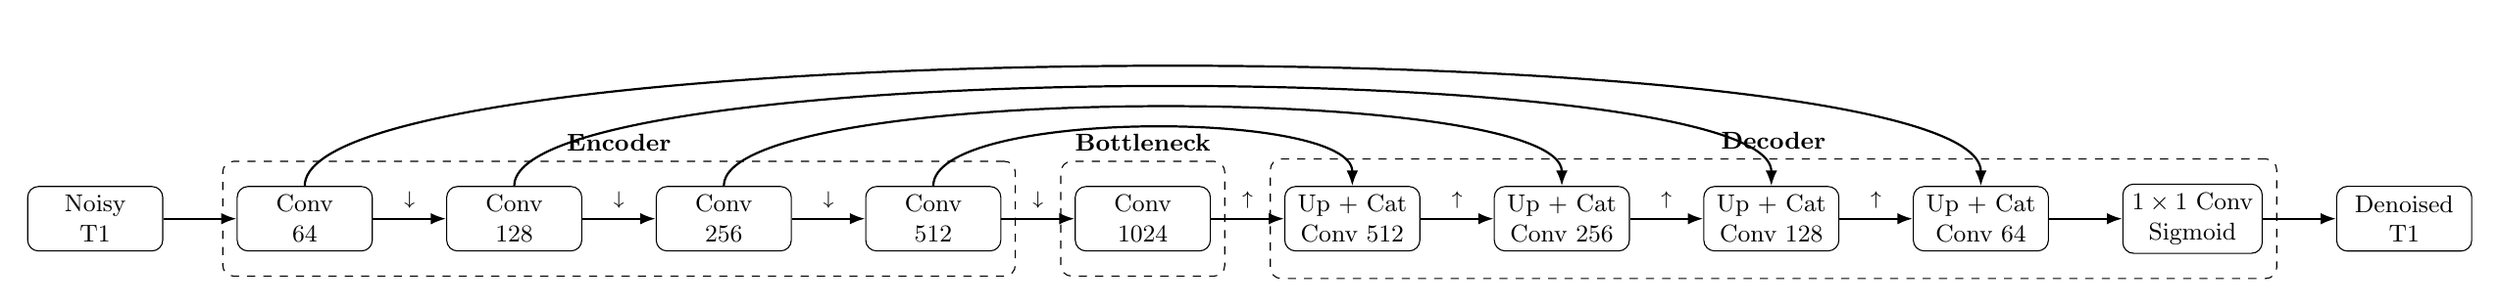
\begin{tikzpicture}[
    node distance=0.95cm,
    block/.style={
        draw,
        rounded corners,
        minimum width=1.75cm,
        minimum height=0.75cm,
        align=center,
        font=\small
    },
    io/.style={
        draw,
        rounded corners,
        minimum width=1.75cm,
        minimum height=0.75cm,
        align=center,
        font=\small
    },
    arrow/.style={-{Latex[length=2mm]}, thick},
    skip/.style={-{Latex[length=2mm]}, thick}
]

\node[io] (input) {Noisy\\T1};
\node[block, right=of input] (c64) {Conv\\64};
\node[block, right=of c64] (c128) {Conv\\128};
\node[block, right=of c128] (c256) {Conv\\256};
\node[block, right=of c256] (c512) {Conv\\512};
\node[block, right=of c512] (c1024) {Conv\\1024};

\node[block, right=of c1024] (u512) {Up + Cat\\Conv 512};
\node[block, right=of u512] (u256) {Up + Cat\\Conv 256};
\node[block, right=of u256] (u128) {Up + Cat\\Conv 128};
\node[block, right=of u128] (u64) {Up + Cat\\Conv 64};
\node[block, right=of u64] (outconv) {$1\times1$ Conv\\Sigmoid};
\node[io, right=of outconv] (output) {Denoised\\T1};

\draw[arrow] (input) -- (c64);
\draw[arrow] (c64) -- node[above, font=\scriptsize] {$\downarrow$} (c128);
\draw[arrow] (c128) -- node[above, font=\scriptsize] {$\downarrow$} (c256);
\draw[arrow] (c256) -- node[above, font=\scriptsize] {$\downarrow$} (c512);
\draw[arrow] (c512) -- node[above, font=\scriptsize] {$\downarrow$} (c1024);
\draw[arrow] (c1024) -- node[above, font=\scriptsize] {$\uparrow$} (u512);
\draw[arrow] (u512) -- node[above, font=\scriptsize] {$\uparrow$} (u256);
\draw[arrow] (u256) -- node[above, font=\scriptsize] {$\uparrow$} (u128);
\draw[arrow] (u128) -- node[above, font=\scriptsize] {$\uparrow$} (u64);
\draw[arrow] (u64) -- (outconv);
\draw[arrow] (outconv) -- (output);

\draw[skip] (c512.north) .. controls +(0,1.0) and +(0,1.0) .. (u512.north);
\draw[skip] (c256.north) .. controls +(0,1.35) and +(0,1.35) .. (u256.north);
\draw[skip] (c128.north) .. controls +(0,1.7) and +(0,1.7) .. (u128.north);
\draw[skip] (c64.north) .. controls +(0,2.05) and +(0,2.05) .. (u64.north);

\begin{scope}[on background layer]
\node[
    draw,
    dashed,
    rounded corners,
    inner xsep=0.18cm,
    inner ysep=0.32cm,
    fit=(c64)(c128)(c256)(c512),
    label={[font=\small\bfseries]above:Encoder}
] (encoderbox) {};

\node[
    draw,
    dashed,
    rounded corners,
    inner xsep=0.18cm,
    inner ysep=0.32cm,
    fit=(c1024),
    label={[font=\small\bfseries]above:Bottleneck}
] (bottleneckbox) {};

\node[
    draw,
    dashed,
    rounded corners,
    inner xsep=0.18cm,
    inner ysep=0.32cm,
    fit=(u512)(u256)(u128)(u64)(outconv),
    label={[font=\small\bfseries]above:Decoder}
] (decoderbox) {};
\end{scope}

\end{tikzpicture}
}
\caption{2D U-Net 网络结构示意}
\label{fig:unet_arch}
\end{figure}

从结构上看，编码器路径用于逐步提取更高层的上下文特征，解码器路径用于恢复图像的空间分辨率。跳跃连接是该结构中的关键部分，它将高分辨率的浅层特征直接传递到对应的解码阶段，使模型在进行噪声抑制的同时能够更好地保留脑组织边缘和局部纹理。由于本实验输入输出均为单通道二维切片，因此 2D U-Net 能够在相对较低的工程复杂度下，完成对 MRI 切片图像的去噪任务。

\subsection{损失函数与评价指标}

训练损失由 L1 损失与 SSIM 损失加权组成。下面依次给出两者的定义。

首先给出 L1 损失的定义。设输入 noisy 切片为 $x$，对应 clean 切片为 $y$，模型输出为 $\hat{y}=f_{\theta}(x)$。L1 损失定义为
\begin{equation}
\mathcal{L}_{L1}=\frac{1}{N}\sum_{i=1}^{N}|\hat{y}_i-y_i| ,
\end{equation}
其中 $N$ 表示切片中的像素总数。L1 损失直接约束预测图像与干净图像之间的逐像素绝对误差，相比 MSE 对少量较大误差更不敏感，适合医学图像重建中的灰度保真任务。

接着给出 SSIM 损失的定义。SSIM 用于衡量两幅图像在亮度、对比度和结构上的相似程度，其基本形式为
\begin{equation}
\operatorname{SSIM}(\hat{y},y)=
\frac{(2\mu_{\hat{y}}\mu_y+C_1)(2\sigma_{\hat{y}y}+C_2)}
{(\mu_{\hat{y}}^2+\mu_y^2+C_1)(\sigma_{\hat{y}}^2+\sigma_y^2+C_2)} .
\end{equation}
其中 $\mu_{\hat{y}}$ 与 $\mu_y$ 表示局部均值，$\sigma_{\hat{y}}^2$ 与 $\sigma_y^2$ 表示局部方差，$\sigma_{\hat{y}y}$ 表示局部协方差。实验中 SSIM 在 $11\times11$ 高斯滑窗上计算，高斯核标准差为 1.5，常数项设置为 $C_1=(0.01)^2$、$C_2=(0.03)^2$。由于训练目标需要最小化损失，因此 SSIM 损失定义为
\begin{equation}
\mathcal{L}_{SSIM}=1-\operatorname{SSIM}(\hat{y},y).
\end{equation}

综合 L1 损失与 SSIM 损失，给出最终联合损失的定义：
\begin{equation}
\mathcal{L}=\mathcal{L}_{L1}+0.5\mathcal{L}_{SSIM}.
\end{equation}
这一加权组合使模型同时关注像素级强度误差和局部结构一致性。若只使用像素级损失，模型可能在数值误差上表现较好，但结构边缘被过度平滑；加入 SSIM 损失后，训练目标能够更直接地约束去噪结果与 clean 图像在结构上的相似程度。

测试阶段主要使用 PSNR 与 SSIM 评价去噪效果。PSNR 基于均方误差计算，定义为
\begin{equation}
\operatorname{MSE}=\frac{1}{N}\sum_{i=1}^{N}(\hat{y}_i-y_i)^2 ,
\end{equation}
\begin{equation}
\operatorname{PSNR}=10\log_{10}\left(\frac{MAX_I^2}{\operatorname{MSE}}\right).
\end{equation}
由于图像已归一化到 $[0,1]$，因此 $MAX_I=1$。PSNR 越高，说明预测图像与 clean 图像之间的均方误差越小；SSIM 越接近 1，说明两幅图像的结构相似性越高。需要说明的是，$100.00\,\mathrm{dB}$ 为 PSNR 计算的数值上界，由 MSE 防除零截断（$1\times10^{-10}$）导致。当预测切片中背景区域占比高且误差极小时，PSNR 会达到这一饱和值。

\subsection{实验设置}

优化器采用 Adam，学习率为 $1.0\times10^{-4}$，batch size 为 16，最大训练轮数为 50，不启用权重衰减。训练过程中使用随机水平翻转作为数据增强，noisy 与 clean 切片同步翻转，以保证监督目标仍然与输入图像空间对齐。早停策略基于验证集 PSNR 设置，若连续 10 个 epoch 验证集 PSNR 未刷新最高记录，则停止训练。训练过程中保存验证集 PSNR 最优的 checkpoint，同时保存最近一个 epoch 的 last checkpoint，以便后续恢复训练。

需要说明的是，本实验包含两次连续训练运行。Run 1 从随机初始化开始训练，训练至第 24 个 epoch 时，由于验证集 PSNR 连续 10 个 epoch 未刷新最高记录而触发早停。由于距离预设的 50 epoch 上限较远，Run 2 基于第 24 个 epoch 结束时保存的 \texttt{last.pt} 权重进行续训，且不参考 Run 1 的最佳权重。Run 2 从第 25 个 epoch 继续至第 36 个 epoch，并再次触发早停。鉴于 Run 2 保留了 Run 1 的早停设置，可以确认 Run 2 在第 26 个 epoch 已达到最优。续跑中出现的这一快速收敛现象，进一步验证了 Run 1 最优结果的可靠性。

\section{实验结果与分析}

\subsection{模型性能评价}

下表为两次训练运行在各自最优 epoch 上的训练集、验证集及测试集核心指标汇总。

\begin{table}[H]
\centering
\caption{两次训练运行的最优指标汇总}
\begin{tabular}{lccc}
\toprule
运行 & Slice PSNR (train/val/test) & Slice SSIM (train/val/test) & Case PSNR/SSIM (test) \\
\midrule
Run 1 & 71.37/100.00/100.00 dB & 0.9947/0.9921/0.9925 & 45.34 dB/0.9897 \\
Run 2 & 69.67/97.08/97.07 dB & 0.9949/0.9908/0.9912 & 45.35 dB/0.9881 \\
\bottomrule
\end{tabular}
\end{table}

由表 1 可知，两个 run 在 slice 级口径下均取得较高的重建指标。训练、验证与测试 slice PSNR 均处于较高水平(训练集 slice PSNR 显著低于验证集与测试集，系切片更多、难度分布更广所致，不代表重建质量更差)。slice SSIM 也基本维持在 0.99 左右，说明模型在单张切片层面能够较好恢复 clean T1 图像强度分布与局部结构。不过，slice 级均值不足以代表完整三维 case 的整体去噪质量。一方面，不同 case 包含的有效切片数不同，直接汇总 slice 结果会使切片多的 case 在均值中占据更高权重；另一方面，slice 级 PSNR 容易受到低误差切片和背景区域的数值放大影响。因此仍需要 case 级指标作为性能佐证。

在 case 级测试口径下，Run 1 的 PSNR 为 45.34 dB、SSIM 为 0.9897，Run 2 的 PSNR 为 45.35 dB、SSIM 为 0.9881。从绝对数值看，45 dB 左右的 PSNR 表明预测图像与 clean 图像之间的重建误差已经较低，接近 0.99 的 SSIM 也说明模型在去噪后仍能较好保留脑部结构信息。从两次运行的一致性看，二者的 PSNR 仅相差 0.01 dB，SSIM 差异也较小，说明模型不仅在训练集与验证集上表现稳定，在完整测试 case 上的去噪性能也已基本收敛。总体而言，表 1 说明该 2D U-Net 不仅能够取得较高的测试集去噪质量，而且其最终性能在两次训练运行之间具有较好一致性。

\subsection{训练曲线分析}

下图为模型训练与验证损失曲线，其中第 1 个 epoch 以 batch 级曲线呈现(每 5 个 batch 记录一个点)，第 2 至第 36 个 epoch 以 epoch 级曲线呈现。

\begin{figure}[H]
\centering
\maybeincludegraphics[width=0.98\linewidth]{P1_losses.png}
\caption{训练与验证损失曲线}
\label{fig:loss_curves}
\end{figure}

由图可知，模型在第 1 个 epoch 内经历了快速收敛。总损失从约 0.58 快速下降到接近 0.006，L1 损失从约 0.23 降至接近 0.003，SSIM 损失也从约 0.70 降至接近 0.006。进一步观察该 epoch 内部的 batch 级曲线可以发现，主要下降集中在第 1 个 epoch 的前三分之一部分(约 1500 batch)，随后曲线已接近低损失区间并进入小幅波动状态。三个指标在这一阶段同步下降，说明模型并不是只降低了某一种损失项，而是在像素强度重建和局部结构相似性两个层面同时获得了明显改善。这说明模型从随机初始化开始，在第 1 个 epoch 的前三分之一 batch 内就迅速学习到 noisy 与 clean 切片之间的主要映射关系，后续 batch 更多是在已有映射基础上进行局部修正。

从第 2 个 epoch 开始一直到第 36 个 epoch，训练损失即进入缓慢下降阶段。总训练损失整体从约 0.0078 下降到约 0.0051，L1 训练损失从约 0.0041 下降到约 0.0026，SSIM 训练损失从约 0.0075 下降到约 0.0050。相比之下，验证损失没有呈现同样平滑的下降趋势，而是在较窄范围内波动。总验证损失大致处于 0.0055 至 0.0095 区间，L1 验证损失主要集中在 0.0027 至 0.0034 附近，SSIM 验证损失的波动幅度更大，部分 epoch 出现明显尖峰。结合三幅子图对比可以看到，验证端总损失的尖峰与 SSIM 损失的尖峰更为一致，而 L1 验证损失始终保持在较窄区间内。这表明像素级重建误差相对稳定，模型对整体灰度强度的恢复较为可靠；相比之下，结构相似性指标更容易受到不同验证 batch、不同解剖结构切片以及局部边界或纹理差异的影响。

此外，可以观察到 24 epoch 后，即 Run 2 阶段，训练损失仍然维持较低水平且有小幅下降，但验证损失未见持续改善。换言之，续训阶段仍能进一步压低训练目标函数，但这种下降没有同步转化为验证集上的稳定收益。因此，Run 2 的主要作用并不是带来明显的性能跃迁，而是进一步确认模型在 Run 1 后期已经接近稳定收敛状态。结合测试集结果可以进一步确认，继续训练对泛化性能的提升较为有限，后续分析更应关注模型误差的具体形态，而不是单纯延长训练轮数。

整体来看，训练曲线呈现了从快速收敛到稳定精细化的典型特征：第 1 个 epoch 完成了绝大部分损失下降，此后训练损失和验证损失均进入窄幅波动状态，train–val gap 未出现扩大趋势，说明模型未发生明显过拟合。三类损失的行为差异也在这一阶段充分显现：L1 损失极其平稳，SSIM 损失则在验证集上波动更大，提示模型在局部结构保持方面对不同切片或不同解剖区域更为敏感。这种在全局强度重建已经高度准确的前提下、结构级误差仍存在区域差异的现象，自然引出一个进一步的问题：残余误差在空间上究竟是怎样分布的，是否集中在某些特定类型的解剖结构附近。鉴于训练曲线只能反映误差大小和稳定性，不能说明误差具体发生在图像的哪些位置，而 SSIM 损失也只能反映滑动窗口内的整体相似程度，本身不含有详细的空间位置信息，因此需要结合具体切片图像证据对去噪误差的空间分布进行分析。

\subsection{逐切片去噪误差分析}

下图为测试集中 case 级 PSNR 最高与最低的两个 case 的逐切片去噪误差分析。上排对应测试性能最佳的 case 1042186（case PSNR 49.5 dB），下排对应最差的 case 1005669（case PSNR 41.6 dB）。两行均选取各自脑实质区域内像素强度接近该 case 中位数水平的代表切片，以保证对比的公平性。其中，前三列图片分别对应带噪 T1 输入、纯净 T1 参考与模型的去噪输出，均采用灰度显示（黑色为0，白色为1）；第四列为梯度-误差联合编码图，其中颜色编码局部梯度强度（蓝色为平坦区域，红色为锐利解剖边缘），亮度编码纯净参考切片与模型去噪输出切片的逐像素误差绝对值，无梯度且低误差的背景区域被压暗以突出有效区域；第五列为绝对误差热力图，颜色与误差值的映射关系参考右侧颜色标尺。

\begin{figure}[H]
\centering
\maybeincludegraphics[width=0.98\linewidth]{P3_error_analysis.png}
\caption{最佳与最差测试 case 的逐切片去噪误差对比}
\label{fig:error_analysis}
\end{figure}

从前三列的灰度图像对比来看，最佳 case 与最差 case 的 denoised 图像均与 clean 图像保持较高相似度。两组样本中，模型输出都基本恢复了脑组织整体轮廓、脑沟走向、脑室形态和颅骨边缘位置，未出现明显的结构错位、组织缺失或异常伪影。即使在 case 级 PSNR 最低的样本中，denoised 图像在视觉上仍然接近 clean 图像，说明模型的主要问题并不是整体重建失败，而是更细粒度的局部误差。

进一步观察第四列梯度-误差联合编码图可以发现，误差与图像局部结构复杂度明显相关。两组样本中的高误差区域都更容易出现在脑组织外缘、脑沟纹理、灰白质交界以及颅骨边界等局部梯度较高的位置，而较平坦的脑实质和背景区域误差相对较弱。这说明模型对整体强度分布的学习较充分，但在边界锐利、纹理密集或灰度变化较快的区域仍存在一定恢复偏差。该现象也符合去噪任务的特点：模型在抑制噪声时需要在平滑噪声和保留细节之间取得平衡，因此高梯度结构附近更容易成为残余误差集中的位置。

第五列绝对误差热力图更直观地显示了两组 case 的差异。最佳 case 的误差图整体较暗，亮色区域较少，说明预测值与 clean 图像之间的像素差异整体较低，误差主要呈稀疏分布。最差 case 的误差图则出现更大范围的橙黄色点状区域，且这些误差不仅分布在头颅边缘，也延伸到脑实质内部纹理和局部结构复杂区域。这表明最差 case 的较低 PSNR 主要来自低幅度误差在更大空间范围内的累积，而不是少数区域发生严重重建错误。

总体来看，这一可视化结果说明，模型在测试集中能够稳定恢复 T1 图像的主要脑部结构，即使是 case 级 PSNR 最低的样本也没有出现明显结构性失败。最佳 case 与最差 case 的核心差别主要体现在残余误差的范围和强度：前者误差更稀疏、更集中于边界区域，后者误差更弥散，并在脑实质内部细纹理区域出现更多低幅度偏差。因此，本实验模型的主要局限不是整体噪声抑制能力不足，而是在高梯度边界、细粒度纹理和复杂解剖结构附近仍可能出现轻微平滑或残余误差。

\section{总结}

本实验围绕 MRI T1 加权脑部图像去噪任务展开，将带噪 T1 轴向切片到干净 T1 轴向切片的映射建模为监督式图像重建问题。实验流程包括三维 NIfTI 体数据读取、轴向切片提取、脑组织有效切片过滤、分位数归一化、统一尺寸 zero-padding，以及 case 级训练、验证和测试划分。由于数据划分在 case 层面完成，同一受试者的所有切片不会同时出现在不同数据子集中，因此能够避免 slice 级随机划分可能带来的数据泄漏，使测试结果更能反映模型对未见 case 的泛化能力。

方法上，本实验采用 2D U-Net 作为去噪模型。编码器通过下采样提取上下文特征，解码器通过转置卷积恢复空间分辨率，并利用 skip connection 保留高分辨率细节。训练目标采用 L1 损失与 SSIM 损失的加权组合，使模型同时关注像素级灰度保真和局部结构相似性。实验结果表明，两次训练运行在 case 级测试口径下均达到约 45.3 dB 的 PSNR 和约 0.989 的 SSIM，说明模型能够有效降低 T1 图像噪声，并较好保留脑部主要结构。训练曲线也显示，模型在第 1 个 epoch 内完成主要损失下降，随后进入低损失区间内的稳定优化阶段，继续续训带来的泛化收益较为有限。

进一步的逐切片误差可视化显示，最佳 case 与最差 case 的 denoised 图像均与 clean 图像保持较高视觉相似度，未出现明显结构错位、组织缺失或异常伪影。两者差异主要体现在残余误差的范围和强度上：最佳 case 的误差更稀疏，主要集中在局部边界；最差 case 的误差更弥散，并在脑实质内部纹理和复杂结构区域出现更多低幅度偏差。梯度--误差联合图也表明，误差更容易出现在脑组织外缘、脑沟纹理、灰白质交界和颅骨边界等高梯度区域。因此，本实验模型的主要问题不是整体噪声抑制不足，而是在局部边界和细粒度纹理恢复上仍存在一定残余误差。

总体而言，2D U-Net 在本实验设置下能够以相对简洁的结构实现较高质量的 MRI T1 图像去噪，并在测试 case 上保持稳定表现。与此同时，模型仍然只利用单张轴向切片内部信息，没有显式建模相邻切片之间的三维连续性，因此在跨切片连续结构和复杂解剖边界附近可能仍有改进空间。后续工作可以进一步尝试 2.5D 或 3D 网络结构，引入相邻切片上下文，并结合更贴近下游任务或人工判读的评价方式，对去噪结果的实际医学图像分析价值进行更全面评估。

\appendix
\section{代码、模型权重与预测体数据下载链接}

\begin{itemize}
  \item 代码下载Github链接：\url{https://github.com/Jacky23307110248/CS50029-ComputationalNeuroscience/tree/main/PJ2}
  \item 模型权重与预测体数据下载Modelscope链接：\url{https://modelscope.cn/datasets/sSzHox/PJ-denoise}
  \item 训练记录Swanlab链接：\url{https://swanlab.cn/@23307110248JackyH/PJ2/overview}
\end{itemize}

\end{document}
